% !TeX spellcheck = en_EN-English

\section{Embedding of patient}
\label{embeddingRes}

Once again, the first sub-task in predicting a patient’s future costs is to embed each patient record into a numerical vector that can be interpreted by a neural network. Our approach to this process is detailed in Sec. \ref{embeddingImple}. Here, we will examine whether the proposed solution possesses the desired property regarding the similarity between two embeddings.

\subsection{Diagnosis embedding}

We need to confirm that closely related diagnoses receive embeddings with smaller distances-indicating higher similarity-compared to less related diagnoses. To verify that our embeddings exhibit these desired properties, we computed the similarity between embeddings of multiple codes. As our similarity function, we used the simple multiplicative inverse of the Euclidean distance. The results are shown in Tab. \ref{tab:diag_emb_show}. The highest similarity was observed between codes G47.30 and G40.09, which is expected since they belong to the same main category and have very similar subcategories. The second highest similarity was between H40.09 and H18.80, the only other pair belonging to the same main category. This confirms that the main category has the greatest impact, as this similarity is significantly higher than that between G40.09 and H40.09, which differ only in the main category.
\\

\begin{table}[!h]
	\centering
	\begin{tabular}{|l|l|l|}
		\hline
		Code A & Code B & Similarity \\ \hline
		G47.30 & G40.09 & 2.77       \\ \hline
		G47.30 & H40.09 & 0.53       \\ \hline
		G47.30 & H18.80 & 0.46       \\ \hline
		G40.09 & H40.09 & 0.54       \\ \hline
		G40.09 & H18.80 & 0.45       \\ \hline
		H40.09 & H18.80 & 0.84       \\ \hline
	\end{tabular}
	\caption{Similarities of embedding of multiple chosen MKCH-10 codes}
	\label{tab:diag_emb_show}
\end{table}  

Another confirmation that the embeddings function as intended comes from clustering analysis. Specifically, we expect that if we group embeddings into as many clusters as there are main categories, each cluster should contain mostly, if not exclusively, diagnoses from a single main category. To test this, we used K-means clustering with 26 clusters, corresponding to the number of different main diagnosis categories, and obtained the following results:

\begin{table}[!h]
	\centering
	\begin{tabular}{|p{0.15\textwidth}|p{0.2\textwidth}|p{0.5\textwidth}|}
		\hline
		Cluster ID & Cluster size & Frequency of first level values \\ \hline
		0 & 654 & C: 654, \\ \hline
		1 & 2092 & M: 2092, \\ \hline
		2 & 766 & Y: 766, \\ \hline
		3 & 543 & S: 543, \\ \hline
		4 & 786 & Z: 786, \\ \hline
		5 & 1100 & T: 1100, \\ \hline
		6 & 1067 & X: 1067, \\ \hline
		7 & 620 & H: 496, U: 124, \\ \hline
		8 & 752 & S: 752, \\ \hline
		9 & 1770 & M: 1770, \\ \hline
		10 & 739 & Q: 739, \\ \hline
		11 & 584 & D: 584, \\ \hline
		12 & 507 & F: 507, \\ \hline
		13 & 958 & W: 958, \\ \hline
		14 & 556 & E: 556, \\ \hline
		15 & 491 & A: 491, \\ \hline
		16 & 553 & O: 553, \\ \hline
		17 & 627 & K: 627, \\ \hline
		18 & 872 & V: 872, \\ \hline
		19 & 521 & G: 521, \\ \hline
		20 & 463 & L: 463, \\ \hline
		21 & 420 & R: 420, \\ \hline
		22 & 465 & B: 465, \\ \hline
		23 & 717 & J: 319, P: 398, \\ \hline
		24 & 568 & I: 568, \\ \hline
		25 & 535 & N: 535, \\ \hline
	\end{tabular}
	\caption{Size of clusters and frequencies of first level diagnosis codes in them.}
	\label{tab:diag_clusters}
\end{table}

In Tab. \ref{tab:diag_clusters}, we observe that almost every cluster consists of diagnoses from only a single main category. The only immediately visible issues occur in clusters 7 and 23, where two main categories were assigned to the same cluster. This overlap is likely due to their smaller size relative to other categories and the fact that the largest categories (M and S) were split into two clusters.

\subsection{Drug embedding}

To confirm that the desired property of similarity is satisfied also for drug embeddings, we performed a similar check as we did with diagnosis codes. We computed the similarity of four chosen ATC codes and verified if our theory holds. To compute similarity, we again used the multiplicative inverse of Euclidean distance. We selected C01EB15, C01CA04, C10AA07, and J01CA04. We expected the first two to be most similar since they match on the first levels, then the first two compared to the third should have slightly lower similarity since they match on only the first level, and finally, we expected that all three would be least similar to the fourth one since the first level is different, even though the second and fourth match on all other levels except the first. The results are shown in Tab. \ref{tab:drug_emb_show}. We can see that the results met our expectations, with the highest similarity between the first two and the lowest between any of the first three and the fourth, even in the case of the second and fourth that match on all other levels except the first.

\begin{table}[!h]
	\centering
	\begin{tabular}{|l|l|l|}
		\hline
		Code A & Code B & Similarity \\ \hline
		C01EB15 & C01CA04 & 1.24      \\ \hline
		C01EB15 & C10AA07 & 0.54       \\ \hline
		C01EB15 & J01CA04 & 0.45       \\ \hline
		C01CA04 & C10AA07 & 0.64       \\ \hline
		C01CA04 & J01CA04 & 0.48       \\ \hline
		C10AA07 & J01CA04 & 0.38       \\ \hline
	\end{tabular}
	\caption{Similarities of embedding of multiple chosen ATC codes}
	\label{tab:drug_emb_show}
\end{table}  

Similarly to the diagnosis codes, we can test whether our embeddings primarily cluster according to the first level of the code. Since there are 14 main anatomical or pharmacological groups, as shown in Fig. \ref{fig:atc_l1}, we used the K-means algorithm with 14 clusters and obtained the following results:
\\

\begin{table}[!h]
	\centering
	\begin{tabular}{|p{0.15\textwidth}|p{0.2\textwidth}|p{0.5\textwidth}|}
		\hline
		Cluster ID & Cluster size & Frequency of first level values \\ \hline
		0 & 8645 & C: 8645, \\ \hline
		1 & 19132 & N: 19132, \\ \hline
		2 & 9322 & L: 8657, S: 665, \\ \hline
		3 & 11734 & A: 11734, \\ \hline
		4 & 7159 & B: 7159, \\ \hline
		5 & 9526 & V: 9526, \\ \hline
		6 & 4681 & R: 4681, \\ \hline
		7 & 14732 & C: 14732, \\ \hline
		8 & 7237 & V: 7237, \\ \hline
		9 & 4031 & M: 3987, P: 44, \\ \hline
		10 & 3599 & G: 3599, \\ \hline
		11 & 2367 & N: 2367, \\ \hline
		12 & 9032 & D: 1266, G: 897, H: 1136, J: 5733, \\ \hline
		13 & 6093 & N: 6075, P: 18, \\ \hline
	\end{tabular}
\caption{Size of clusters and frequencies of first level drug codes in them.}
\label{tab:drug_clusters}
\end{table}

Based on the results shown in Tab. \ref{tab:drug_clusters}, we conclude that the embeddings generally function as intended. The clusters predominantly consist of embeddings with identical first-level values. Exceptions likely arise from the uneven distribution of drugs across categories. Smaller categories with fewer drugs, such as P, S, D, H, and G, were occasionally assigned to the same cluster as larger categories. Conversely, the largest categories, such as N, C, and V, were split into multiple clusters due to their size. 
\\

These test results confirm that the embeddings operate as designed overall.

\subsection{Medical procedure embedding}

As stated in previous chapters, we tried two different approaches, both using pretrained models. After embedding medical procedure descriptions with both methods, we quickly found that many procedures did not receive any embedding from the Word2vec model. More specifically, 731 out of 7,329 procedures, almost 10\%, were not embedded. Even among the procedures that did receive some embedding, there were many words that were not embedded and therefore did not contribute to the resulting embedding. This was mostly caused by the limitations of the Word2vec model, which can only embed words that are in its dictionary, meaning those available in its training corpus. It seems that many professional medical terms, such as 'polycystické' or 'cytokín', were not present in the corpus. A similar issue could potentially have occurred when using the LaBSE model, however, we found no case where the LaBSE model was unable to embed an entire procedure. Also, thanks to most professional medical terms being similar across multiple languages, and the fact that the LaBSE model was trained on a much larger corpus consisting of 109 distinct languages, it is highly probable that many more terms were successfully embedded, creating a much better embedding of the whole description.
\\

Due to the significant issues with embeddings produced by the Word2vec model, we proceeded exclusively with the LaBSE model, which successfully embedded all procedure descriptions. This model generated 768-dimensional embeddings. To densify the information while retaining most of its content, we applied PCA. We specifically targeted the first few dimensions that would collectively explain over 90\% of variance-a common proxy for preserved information in PCA applications. The algorithm yielded a 119-dimensional embedding that captured 90.4\% of the original embedding's variance.
\\

To validate whether these embeddings effectively encoded procedural semantics, we replicated our drug and diagnosis validation approach using K-means clustering. However, unlike those cases where we had hierarchical code levels for validation, we lacked analogous categorical metadata for procedures. We therefore manually inspected cluster contents to evaluate whether grouped procedures shared meaningful clinical or operational relationships.
\\

Given the 7 329 procedures, we chose K (the number of clusters) to be 365, aiming for approximately 20 procedures per cluster on average. This decision was largely arbitrary. Upon inspecting multiple clusters, we identified many meaningful groupings such as cluster 215, whose procedures are listed in Fig. \ref{fig:G215}, which exclusively contains transplantation-related interventions. However, in some instances, clusters contained a mixture of seemingly unrelated procedures, such as those in cluster 45 shown in Fig. \ref{fig:G45}), which combines the evaluation of final reports with investigations of pharmacokinetics and papillosphincterotomy. Fortunately, it appears that the content of clusters like these is not entirely random but rather consists of multiple subgroups, suggesting that the embedding functions as intended and that we may have simply clustered procedures into too few groups.

\begin{figure}[!h]
	\centering
	
	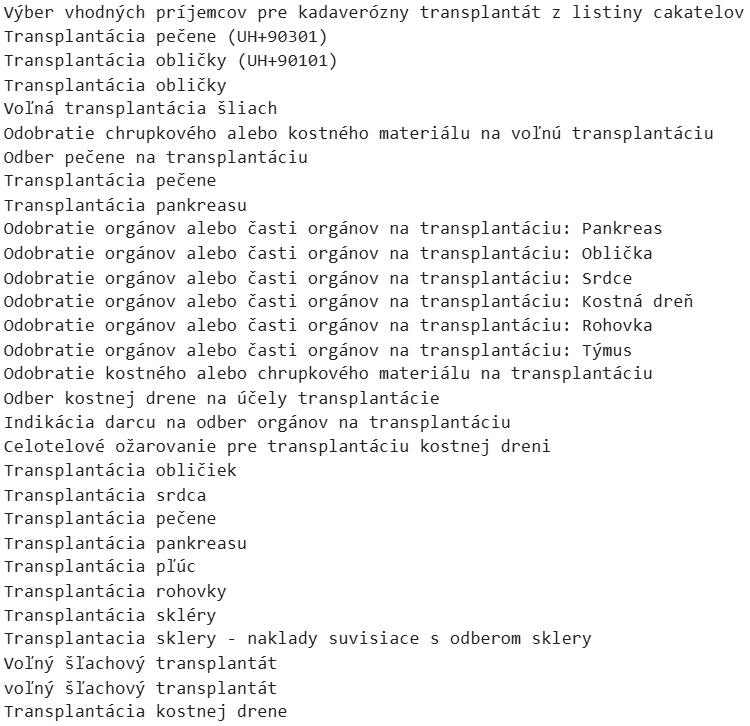
\includegraphics[width=0.6\textwidth]{images/G215.png}
	
	\caption{Medical procedures grouped in cluster number 215.}
	\label{fig:G215}
\end{figure}

\begin{figure}[!h]
	\centering
	
	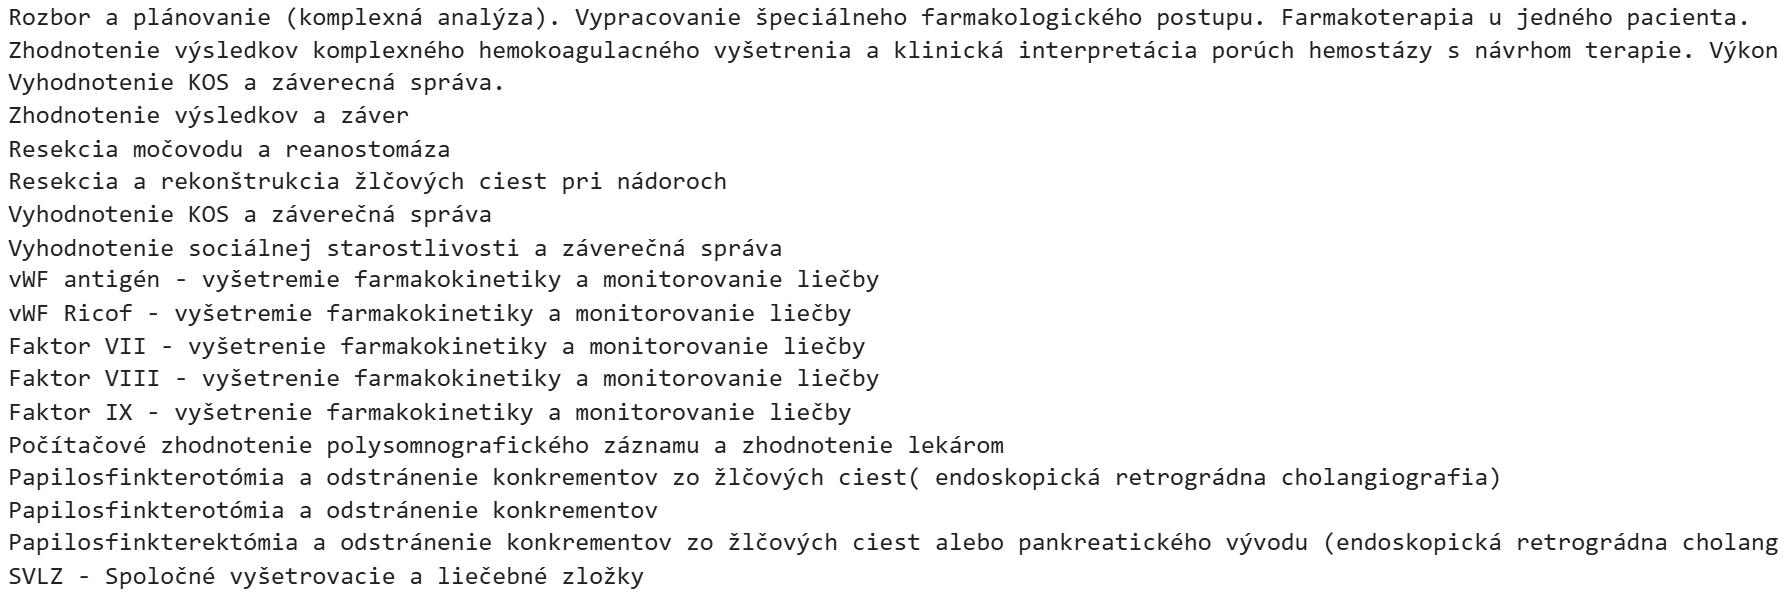
\includegraphics[width=1.1\textwidth]{images/G45.png}
	
	\caption{Medical procedures grouped in cluster number 45.}
	\label{fig:G45}
\end{figure}